\documentclass[journal,12pt,twocolumn]{IEEEtran}
\usepackage{graphicx}
\usepackage{listings}
\usepackage[utf8]{inputenc}
\usepackage{caption}
\usepackage{hyperref}
\usepackage[cmex10]{amsmath}
\usepackage{array}
\usepackage{gensymb}
\usepackage{booktabs}
\usepackage{etoolbox}
\usepackage{amssymb}
\usepackage{datetime} 
\patchcmd{\section}{\centering}{}{}{}
\providecommand{\norm}[1]{\left\lVert#1\right\rVert}
\providecommand{\abs}[1]{\left\vert#1\right\vert}
\let\vec\mathbf

\makeatletter
\newcommand\xleftrightarrow[2][]{%
  \ext@arrow 9999{\longleftrightarrowfill@}{#1}{#2}}
\newcommand\longleftrightarrowfill@{%
  \arrowfill@\leftarrow\relbar\rightarrow}
\makeatother
\title{Optimization}
\author{Somisetty Kedareswari} 
\date{october 2022} 
\newcommand{\myvec}[1]{\ensuremath{\begin{pmatrix}#1\end{pmatrix}}}
\newcommand{\mydet}[1]{\ensuremath{\begin{vmatrix}#1\end{vmatrix}}}
\providecommand{\brak}[1]{\ensuremath{\left(#1\right)}}
\providecommand{\lbrak}[1]{\ensuremath{\left(#1\right.}}
\providecommand{\rbrak}[1]{\ensuremath{\left.#1\right)}}
\providecommand{\sbrak}[1]{\ensuremath{{}\left[#1\right]}}

\begin{document}
\maketitle
\section{Problem Statement}

\noindent A wire of length 28 m is cut into two pieces. One of the pieces to be made in to a square and the other into a circle. What should be the length of each piece so that the combined area of the two is minimum \\

\noindent \textbf{To Find:} \\
The value of the length of each piece so that the combined area of the two is minimum from the two figures that are square and circle.

\noindent \textbf{Given:} \\
Length of the wire is 28m
\section{Construction}
   \begin{center}
  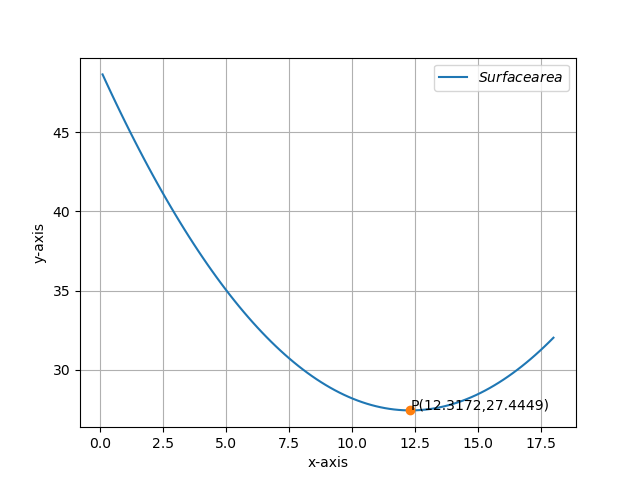
\includegraphics[scale=0.5]{Figure.png}
    \end{center}
\section{solution}
\begin{equation}
\text{length of the circle is} \quad \vec{x} \quad \text{m} .
\end{equation} 
Then length of the other piece for the shape of the square is \begin{equation}
(28-x) \text{m}
\end{equation} 
Perimeter of the square with side a is given by: \\
\begin{equation}
\text{Perimeter of the square = } 4x \\
\label{eq-1}
\end{equation}

\begin{equation}
\text{Circumference of a circle= }2\pi r 
r=\frac{2\pi}{x}
\label{eq-2}
\end{equation}
\begin{equation}
r=\frac{x}{2\pi}
\label{eq-2}
\end{equation}

So, the total length is 
\begin{equation}
4x + 2\pi r = 28
\end{equation} 
The standard equation of the line in conics is given as :
\begin{align}
n^\top \vec{x} = c
\end{align}
\begin{equation}
\begin{pmatrix}4 & 2\pi\end{pmatrix}  \vec{x} = 28
\end{equation}

\begin{align}
\vec{x}  = \myvec{x\\r}
\end{align}
Now by using the formula for the area of the circle and square is:
\begin{equation}
\text{Area of square= }a^2
\end{equation}
\begin{equation}
\text{Area of the circle= }\pi r^2
\end{equation}
Now, the combined area(A) 
\begin{equation}
A=a^2+\pi r^2
\end{equation}
\begin{equation}
A = \frac{x^2}{4\pi} + \frac{(28-x)^2}{4}
\end{equation}
The area of two figures is grepresented as :
\begin{align}
\vec{x}^{\top}\vec{V}\vec{x}+2\vec{u}^{\top}\vec{x}+f=0
\end{align}
\begin{equation}
\vec{V} = \begin{pmatrix}
1 & 0 \\
0 & \pi
\end{pmatrix}
\end{equation}
\begin{equation}
u^\top = \begin{pmatrix}
0 & 0
\end{pmatrix}
\end{equation}
\begin{equation}
f = 0
\end{equation}
\noindent The minimum area is 
\begin{align}
\min_{x} \vec{x}^{\top}\vec{V}\vec{x} 
\end{align}
\section{Calculation of Minima using Gradient Descent algorithm}
\textbf{minima using  Gradient Descent  method}
    \begin{align}
        x_{n+1} &= x_n - \alpha \nabla f(x_n) \\
        \vspace{0.35cm}
        \implies x_{n+1} &= x_n - \alpha\brak{\frac{x}{8}-\frac{28-x}{0.636}}
    \end{align}
\begin{flushleft}
Taking $x_0=0.5,\alpha = 0.001$ and precision = 0.00000001, values obtained using python are:
\end{flushleft} 
\vspace{0.35cm}
\center
        \vspace{0.45cm}
        \boxed{$\text{Minima length of circle} = 12.31$} \\
        \vspace{0.45cm}
        \boxed{$\text{Minimum length of square} = 15.7$ }
\endcenter
\section{Calculation of Minima using CVXPY algorithm}
\textbf{minima using CVXPY method} \\
\noindent Constraint is, 
\begin{equation}
\begin{pmatrix}4& 2\pi\end{pmatrix}  \vec{x} -28 == 0
\end{equation}
Solving using cvxpy, we get
\begin{equation}
\min_{x} \vec{x}^{\top}\vec{V}\vec{x} = 27.45 \quad m^2
\end{equation}
The length of each piece is \\
Circle  = 12.3 m \\
Square = 15.7 m  
\section{Calculation of Minima using Calculus}
 \textbf{minima using conventional method}
    \begin{equation}
        \frac{dA}{dx} = \frac{x^2}{4\pi} + [\frac{28-x}{4}]^2
    \end{equation}
To find minima
    \begin{equation}
	    \frac{dA}{dx} = 0
	    \end{equation}

	    \begin{equation}
\frac{x}{2\pi} + \frac{28-x}{8} = 0
	    \end{equation}
    \begin{equation}
        4x=28\pi-x\pi
    \end{equation}
    \begin{equation}
        x[4+\pi]=28\pi
    \end{equation}
    \begin{equation}
    x=\frac{28\pi}{4+\pi}
    \end{equation}
    The length of each piece is \\
       Circle length =12.3 m  \\
     Square length =15.7 m
\end{document}